\chapter{Diseño e implementación} % Main chapter title

\label{Chapter3} % Change X to a consecutive number; for referencing this chapter elsewhere, use \ref{ChapterX}

\definecolor{mygreen}{rgb}{0,0.6,0}
\definecolor{mygray}{rgb}{0.5,0.5,0.5}
\definecolor{mymauve}{rgb}{0.58,0,0.82}

%%%%%%%%%%%%%%%%%%%%%%%%%%%%%%%%%%%%%%%%%%%%%%%%%%%%%%%%%%%%%%%%%%%%%%%%%%%%%
% parámetros para configurar el formato del código en los entornos lstlisting
%%%%%%%%%%%%%%%%%%%%%%%%%%%%%%%%%%%%%%%%%%%%%%%%%%%%%%%%%%%%%%%%%%%%%%%%%%%%%
\lstset{ %
  backgroundcolor=\color{white},   % choose the background color; you must add \usepackage{color} or \usepackage{xcolor}
  basicstyle=\footnotesize,        % the size of the fonts that are used for the code
  breakatwhitespace=false,         % sets if automatic breaks should only happen at whitespace
  breaklines=true,                 % sets automatic line breaking
  captionpos=b,                    % sets the caption-position to bottom
  commentstyle=\color{mygreen},    % comment style
  deletekeywords={...},            % if you want to delete keywords from the given language
  %escapeinside={\%*}{*)},          % if you want to add LaTeX within your code
  %extendedchars=true,              % lets you use non-ASCII characters; for 8-bits encodings only, does not work with UTF-8
  %frame=single,	                % adds a frame around the code
  keepspaces=true,                 % keeps spaces in text, useful for keeping indentation of code (possibly needs columns=flexible)
  keywordstyle=\color{blue},       % keyword style
  language=[ANSI]C,                % the language of the code
  %otherkeywords={*,...},           % if you want to add more keywords to the set
  numbers=left,                    % where to put the line-numbers; possible values are (none, left, right)
  numbersep=5pt,                   % how far the line-numbers are from the code
  numberstyle=\tiny\color{mygray}, % the style that is used for the line-numbers
  rulecolor=\color{black},         % if not set, the frame-color may be changed on line-breaks within not-black text (e.g. comments (green here))
  showspaces=false,                % show spaces everywhere adding particular underscores; it overrides 'showstringspaces'
  showstringspaces=false,          % underline spaces within strings only
  showtabs=false,                  % show tabs within strings adding particular underscores
  stepnumber=1,                    % the step between two line-numbers. If it's 1, each line will be numbered
  stringstyle=\color{mymauve},     % string literal style
  tabsize=2,	                   % sets default tabsize to 2 spaces
  title=\lstname,                  % show the filename of files included with \lstinputlisting; also try caption instead of title
  morecomment=[s]{/*}{*/}
}


%----------------------------------------------------------------------------------------
%	SECTION 1
%----------------------------------------------------------------------------------------

En este capítulo se exponen los detalles del diseño de los dispositivos primario y secundarios, se describe el desarrollo y funcionamiento del hardware, software y las características más resaltantes del proyecto.

\section{Sistemas complejos de detección de incendios}

Un sistema de detección de incendio no se limita a un único edificio, en instalaciones de mayor escala es común observar sistemas compuestos por más de un edificio, donde se requiere del monitoreo de áreas comunes o incluso zonas que son de particular interés para el tópico de alarmas de incendio, como por ejemplo depósito de materiales inflamables, generadores eléctricos de respaldo o sistema de bombeo de extinción.

En este nivel los sistemas suelen estar compuestos por más de una central de alarma de incendio, las cuales pueden interconectadas entre sí y formar una red de dispositivos de detección, dependiendo del nivel de integración, los sistemas pueden tener total independencia o por el contrario funcionar como una única unidad de detección, por lo que  no siempre es una tarea sencilla identificar la ubicación de origen de un evento.

Un ejemplo de una instalación con potencial para un sistema de detección de incendio complejo puede observarse en la figura \ref{fig:figura_a3}, donde podemos observar una propiedad compuesta por tres edificios y una zona crítica, con una posible estructura de dispositivos primarios y secundarios que permite definir el estado del sistema de detección de incendio en su totalidad.


\begin{figure}[]
	\centering
	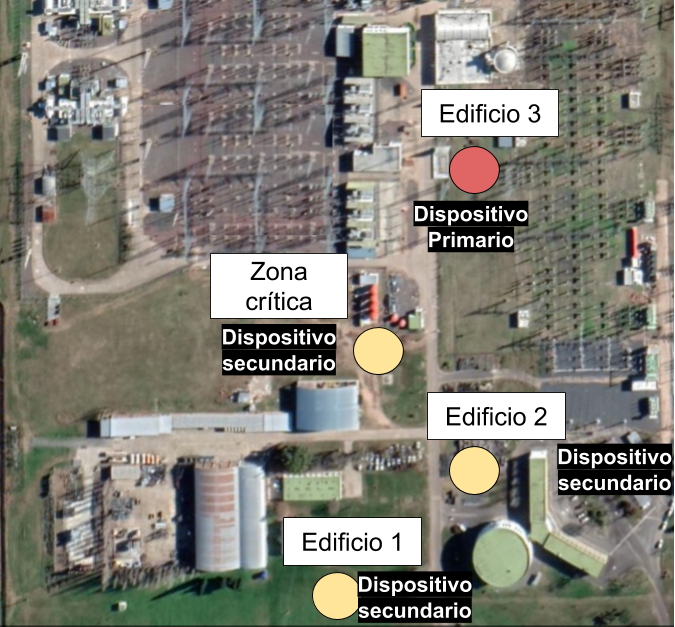
\includegraphics[scale=.25]{./Figures/Capitulo3/Fig_A3.png}
	\caption{Ejemplo de sistema de detección de incendio complejo.}
	\label{fig:figura_a3}
\end{figure}

\section{Criterios de diseño}

El sistema corresponde al primero de una serie de proyectos que tienen como objetivo la generación de alternativas de monitoreo de sistemas de detección de incendio, en esta etapa el objetivo propuesto es adquirir únicamente el estado de la instalación, pero en futuros proyectos se desea alcanzar un mayor nivel de detalle, a continuación se describen los criterios considerados para la selección de los componentes:

Escalabilidad: El sistema debe contar con los recursos necesarios para la integración de nuevas funcionalidades o servicios.

Robustez: Una característica que se desea proporcionar a los sistemas es la posibilidad de tener formas alternativas de trabajo ante eventos de falla.

Recuperabilidad: El mantenimiento de equipos de detección de incendio suele realizarse de forma mensual, por lo que el sistema debe estar en capacidad de restituirse de forma automática en caso de fallas, para evitar visitas adicionales por fallas del dispositivo de monitoreo.

Documentación adecuada:  El sistema debe desarrollarse a partir de plataformas con documentación detallada y de fácil acceso.

Disponibilidad en el mercado Argentino: Los sistemas deberán estar compuestos por elementos que puedan ser adquiridos en el mercado local.

\subsubsection{Criterios fundamentales}

Es de suma importancia respetar dos criterios principales:
\begin{itemize}
\item La no afectación la secuencia de accionamiento de la central de forma remota. 
\item El sistema de monitoreo no debe utilizarse como un dispositivo de detección de incendio.
\end{itemize}

En la figura \ref{fig:figura_b3} podemos observar esquemas de conexión y el uso recomendado del sistema de monitoreo.

\begin{figure}[]
	\centering
	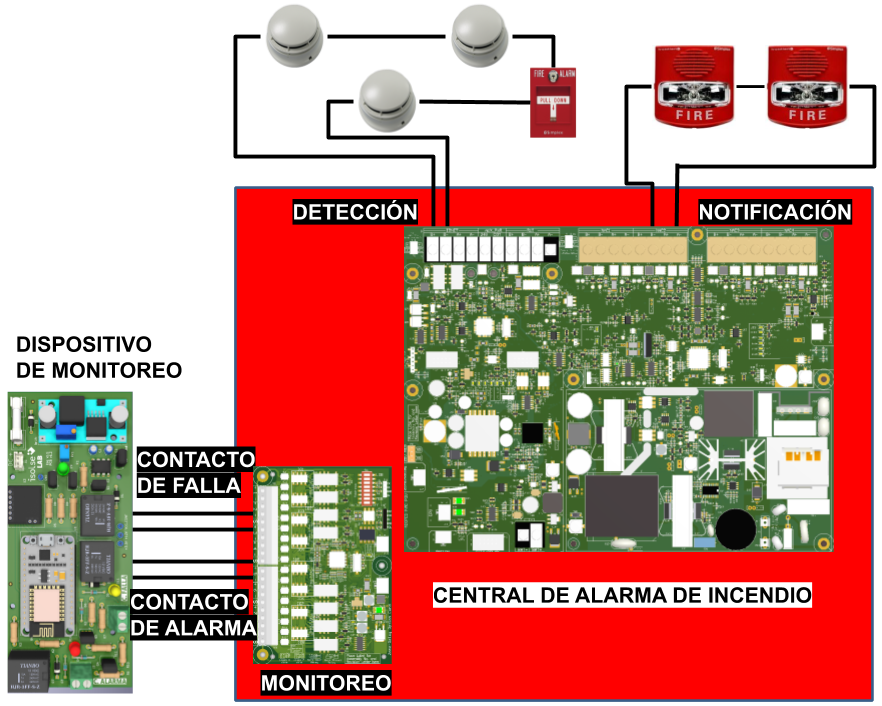
\includegraphics[scale=.25]{./Figures/Capitulo3/Fig_B3.png}
	\caption{Esquema de conexión entre dispositivo de monitoreo y central de alarma de incendio.}
	\label{fig:figura_b3}
\end{figure}

\section{Arquitectura general del sistema}

En esta fase se procede a describir los elementos que componen el sistema de monitoreo, su funcionamiento y la interconexión entre los mismos.


\subsection{Dispositivo primario} 

El dispositivo primario cuenta con los recursos necesarios para el monitoreo de un sistema de detección de alarma base, compuesto por una única central de alarma de incendio a monitorear. El dispositivo implementa un monitoreo periodico a los contactos de alarma y falla para determinar el estado del equipo local, el siguiente paso es facilitar esta información al usuario, para lo que hace uso de tres recursos de notificación:
\begin{itemize}
\item Leds de indicación de estado.
\item Interfaz web para notificación local, por medio de la plataforma Node-RED.
\item Servidor web firebase.
\end{itemize}

A pesar de ser un dispositivo para el monitoreo de un sistema de detección de alarma base, este dispositivo considera la posibilidad de un sistema de detección complejo, para lo que dispone de un módulo específico para la gestión de comunicación inalámbrica, que permite al sistema comunicarse con diferentes dispositivos de monitoreo secundarios, cuyo objetivo principal es reportar el estado de cada subsistema o equipo que se desee monitorear.

Si el dispositivo se va emplear para sistemas complejos de detección, el dispositivo primario procesa el estado local y los estados remotos para generar un diagnóstico del sistema de detección en general, de esta forma en caso de no existir vinculación entre los equipos de detección de alarma el sistema es capaz de establecer el estado correcto de la instalación en su totalidad.

En la figura \ref{fig:figura_c3} se presenta el diseño general del dispositivo primario. 

\begin{figure}[]
	\centering
	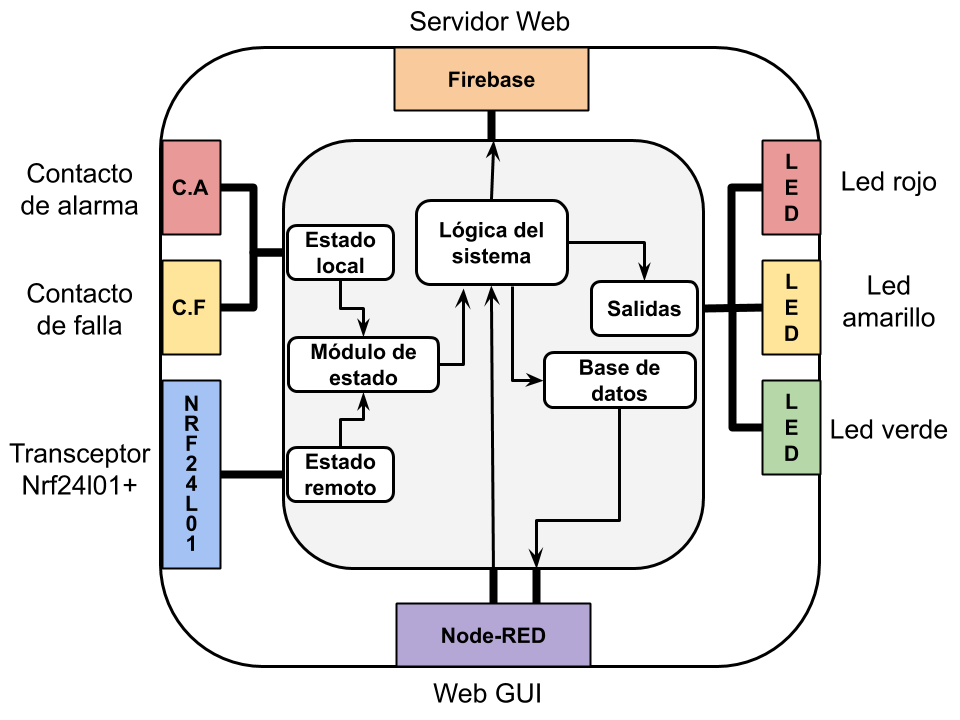
\includegraphics[scale=.25]{./Figures/Capitulo3/Fig_C3.png}
	\caption{Arquitectura del dispositivo primario.}
	\label{fig:figura_c3}
\end{figure}

\subsection{Dispositivo secundario}

El dispositivo secundario realiza el  monitoreo de los contactos de alarma y falla, cuenta con módulo destinado a la gestión de la transmisión de información mediante comunicación inalámbrica. El sistema presenta la información al usuario mediante tres leds de colores específicos, rojo para alarma, amarillo para fallas y verde para normal.


Incluir en el diseño un dispositivo secundario permite incluir un equipo adicional a monitorear, y además incrementa el alcance de la comunicación inalámbrica, ya que cada nodo actúa como nodo-repetidor. En la figura \ref{fig:figura_d3} se observa el diseño general del dispositivo secundario.


\begin{figure}[]
	\centering
	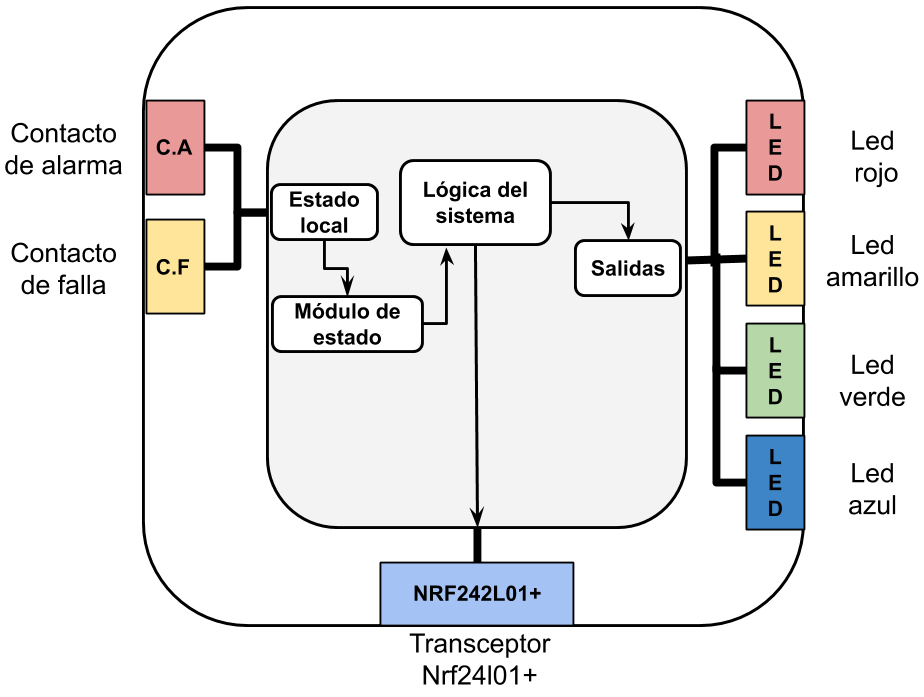
\includegraphics[scale=.25]{./Figures/Capitulo3/Fig_D3.png}
	\caption{Arquitectura del dispositivo secundario.}
	\label{fig:figura_d3}
\end{figure} 

\subsection{Aplicación en sistemas de detección complejos}

Una instalación como la descrita en la figura \ref{fig:figura_a3}, compuesto por tres edificios y una zona crítica, puede ser monitoreado con una estructura como la dispuesta en la figura \ref{fig:figura_e3}, donde podemos observar las interfaces entre los elementos del sistema,  y cómo se relacionan entre ellos.

\begin{figure}[]
	\centering
	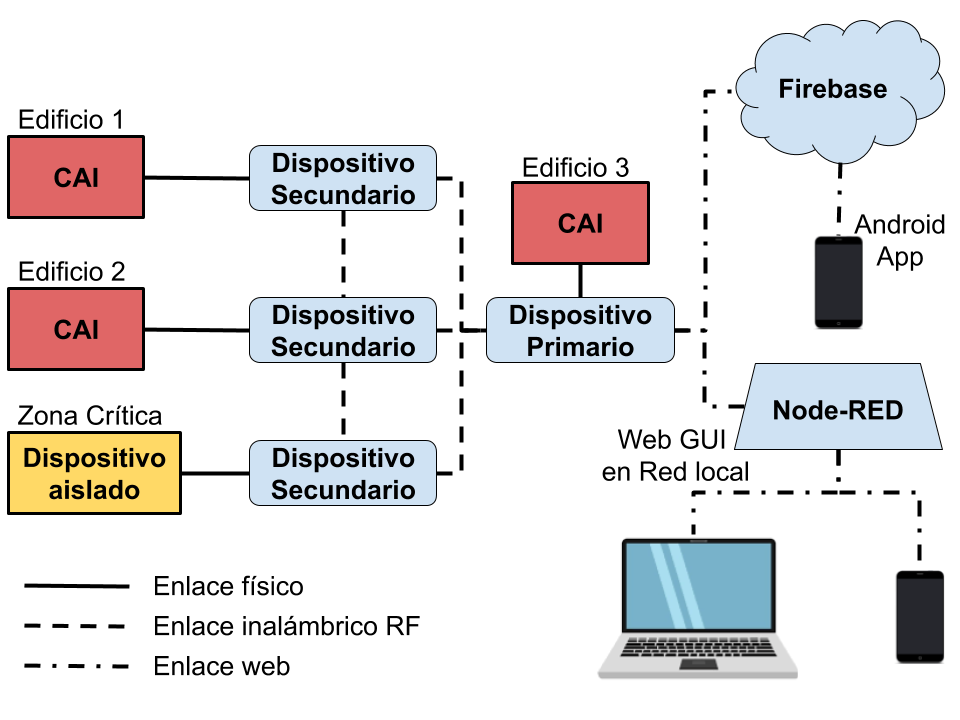
\includegraphics[scale=.25]{./Figures/Capitulo3/Fig_E3.png}
	\caption{Arquitectura general del dispositivo de monitoreo remoto.}
	\label{fig:figura_e3}
\end{figure} 

\section{Hardware}

Esta sección describe el  diseño del hardware utilizado para los dispositivos primario y secundario, sus características, módulos internos y la relación entre ellos.

\subsection{Hardware del dispositivo primario}

Las figuras \ref{fig:figura_f3}, \ref{fig:figura_g3} y \ref{fig:figura_h3}, muestran los esquemáticos empleados para la implementación del hardware del dispositivo primario. El diseño fue concretado como un poncho para la Raspberry Pi, compuesto por los siguientes módulos:

\subsubsection{Módulo de monitoreo de contactos secos}

El diseño de este módulo hace uso de los contactos normal abierto del dispositivo a monitorear para la indicación de alarma o falla en el sistema. La indicación correspondiente se hace a través del accionamiento de un relé interno que modifica el estado del circuito asociado.
La figura \ref{fig:figura_f3} muestra el esquema del módulo de monitoreo de contacto secos.

\begin{figure}[]
	\centering
	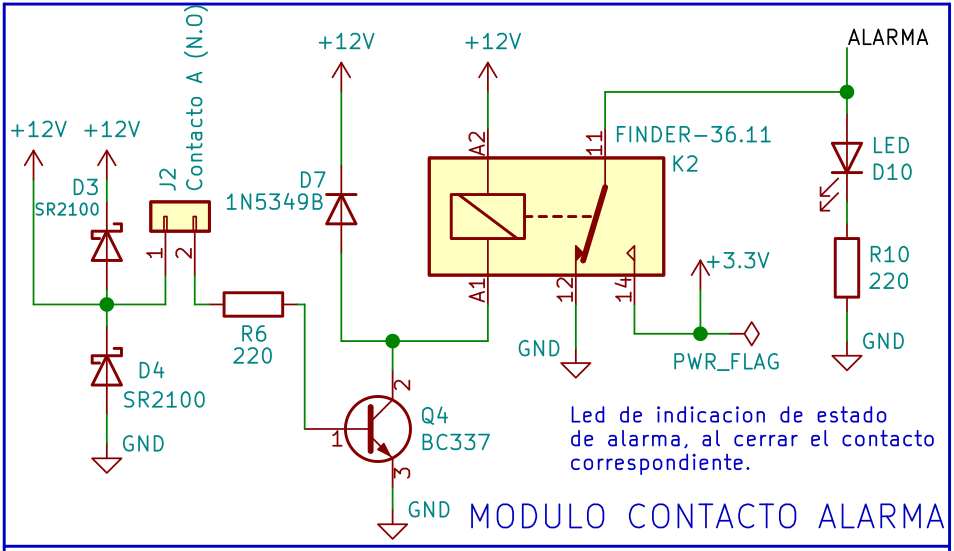
\includegraphics[scale=.25]{./Figures/Capitulo3/Fig_F3.png}
	\caption{Módulo de monitoreo de contacto seco de alarma.}
	\label{fig:figura_f3}
\end{figure} 

El diseño considera la posibilidad de ocurrencia de un error de conexión, para lo cual se incluyó una etapa de protección, que se encarga de mantener la tensión dentro de los rangos de trabajo del dispositivo [0 - 12] vdc.

\subsubsection{Módulo de comunicación nrf24l01+.}

La conexión del módulo transceptor nrf24l01+ se hace siguiendo el esquema recomendado [bibliografía], como puede observarse en la figura \ref{fig:figura_g3}, consiste en una conexión directa con el dispositivo y alimentado por la fuente de 3.3 vdc del dispositivo primario.  

\begin{figure}[]
	\centering
	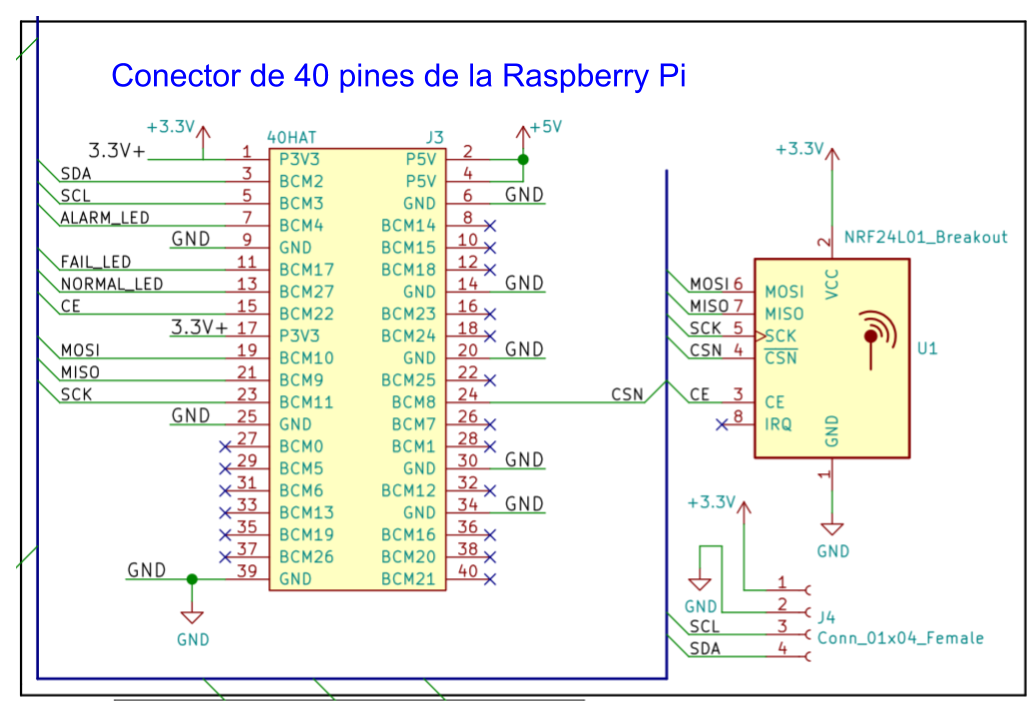
\includegraphics[scale=.25]{./Figures/Capitulo3/Fig_G3.png}
	\caption{Módulo de comunicación inalámbrica.}
	\label{fig:figura_g3}
\end{figure} 

\subsubsection{Módulo de notificación visual}

La notificación visual sigue lo establecido por los requerimientos  ......... y permite al  dispositivo reportar el estado del sistema a monitorear de forma local, sin necesidad de dispositivos adicionales. En la figura \ref{fig:figura_h3} se presentan las conexiones y pines utilizados por el sistema.

\begin{figure}[]
	\centering
	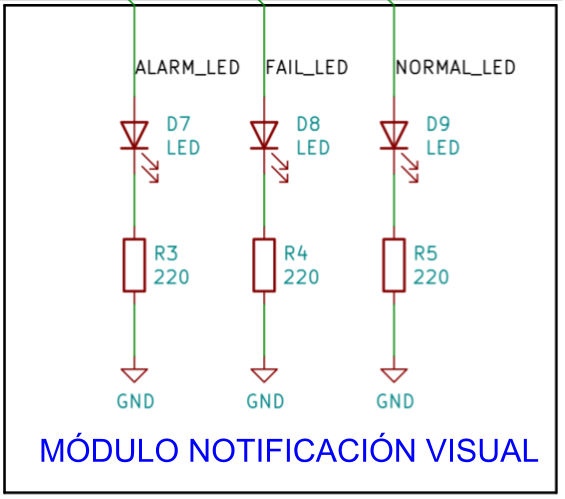
\includegraphics[scale=.25]{./Figures/Capitulo3/Fig_H3.png}
	\caption{Módulo de notificación visual.}
	\label{fig:figura_h3}
\end{figure} 


\subsection{Hardware del dispositivo secundario}

El diseño del sistema puede observarse en las figuras \ref{fig:figura_j3},\ref{fig:figura_k3},\ref{fig:figura_l3},\ref{fig:figura_m3}, se reutiliza el diseño de la figura \ref{fig:figura_f3} para el monitoreo de contactos y añaden al sistema los módulos descritos a continuación.

\subsubsection{Módulo de comunicación nrf24l01+ con amplificador de potencia}

El dispositivo secundario utiliza un módulo nrf24l01+ con un amplificador de potencia, por lo que a diferencia del dispositivo primario, se utiliza un adaptador para la conexión del módulo que garantiza una tensión de alimentación estable. El esquema de conexión se detalla en la figura \ref{fig:figura_j3}.

\begin{figure}[]
	\centering
	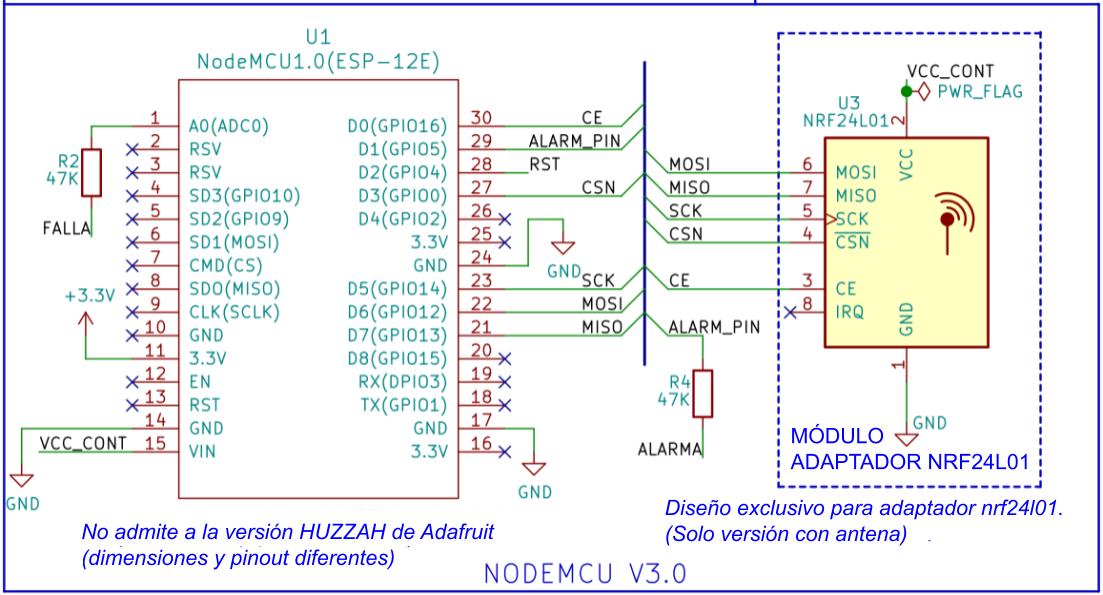
\includegraphics[scale=.25]{./Figures/Capitulo3/Fig_J3.png}
	\caption{Módulo de comunicación inalámbrica de largo alcance.}
	\label{fig:figura_j3}
\end{figure} 


\subsubsection{Módulo de notificación visual}

Debido a restricciones del dispositivo con respecto al número de GPIOS disponibles, el sistema no implementa una conexión directa con el led de notificación de estado normal, en la figura \ref{fig:figura_k3} se puede verificar que el encendido del led indicador del estado normal, se realiza a través de hardware ante la ausencia de señales de falla o alarma.

\begin{figure}[]
	\centering
	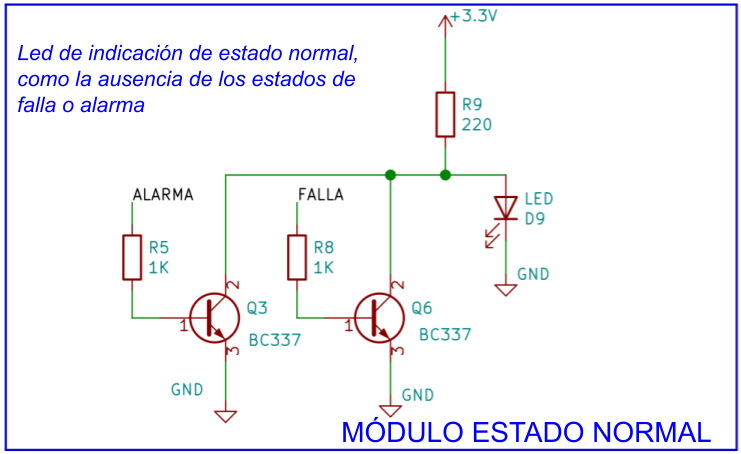
\includegraphics[scale=.25]{./Figures/Capitulo3/Fig_K3.png}
	\caption{Módulo de notificación visual.}
	\label{fig:figura_k3}
\end{figure} 


\subsubsection{Módulo de alimentación}

La alimentación del dispositivo se obtiene a partir del módulo LM2596S-123-3000, un regulador de tensión continua regulable, configurado a 12 vdc. La figura \ref{fig:figura_l3} exhibe al módulo de alimentación y el diseño de una etapa de protección ante casos de conexión con polaridad inversa.

\begin{figure}[]
	\centering
	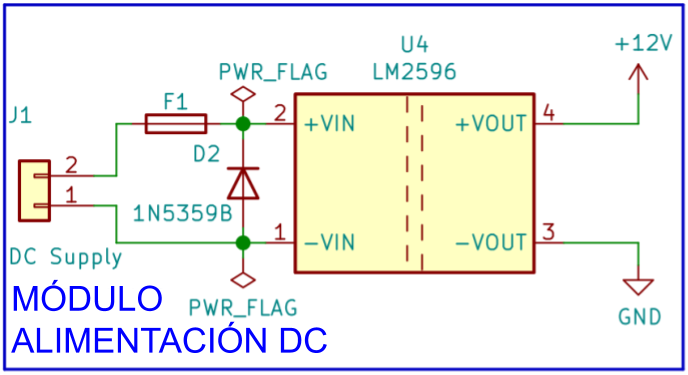
\includegraphics[scale=.25]{./Figures/Capitulo3/Fig_L3.png}
	\caption{Módulo de notificación visual.}
	\label{fig:figura_k3}
\end{figure} 


\section{Software}

